\section{Les lampes à lave (5 points)}

Certaines boutiques vendent des lampes décoratives, appelées <<lampes à lave>>. La chaleur dégagée par l'ampoule située dans le pied de la lampe fait fondre une cire colorée solide. Celle-ci se déplace alors dans une colonne contenant de l'alcool.

\begin{multicols}{2}
	\begin{questions}
		\question[1\half] La cire solide est-elle soluble dans l'alcool ?
		
		\question[1\half] Quel changement d'état subit la cire lorsque la lampe fonctionne ?
		
		\question[2] L'alcool et la cire sont-ils miscibles ?
	\end{questions}

	\begin{center}
		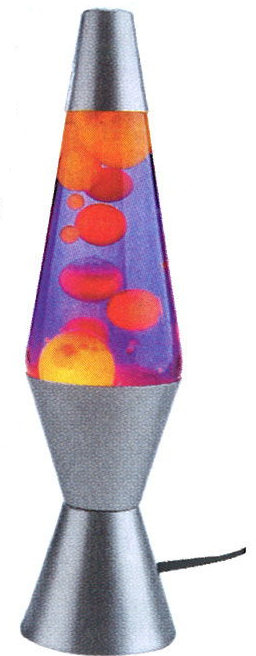
\includegraphics[scale=0.8]{img/lampe}
	\end{center}
\end{multicols}